\chapter{Shluková analýza} \label{sec:clusteranalysis}
Shluková analýza je možná jeden z~nevíce zkoumaných problémů v~oblasti strojového učení a~dolování dat~\cite{Aggarwal13}. Lze ji využít ve velkém množství oborů a~disciplín jako například sumarizace a~segmentace dat, cílený marketing a~nebo již zmíněné strojové učení~\cite{Jain10, Kaufman90}. Základní problém shlukování můžeme formulovat následovně: \textit{Máme množinu vstupních bodů, snažíme se je rozdělit tak, aby skupiny obsahovaly co nejpodobnější body.} Tato formulace je záměrně vágní, protože se různé definice problému velice liší v~závislosti na specifických vlastnostech dat, které se snažíme zařadit do shluků~\cite{Aggarwal13}. 

\section{Definice}
Jelikož je shluková analýza velmi různorodá, zahrnuje mnoho algoritmů, které se mohou značně lišit, protože závisí na datovém modelu a~konkrétní úloze~\cite{Aggarwal13}. Velice se také liší v~definici shluku a~v metodách hledání shluků. Mezi nejčastější definice shluků patří například shluky s~malou vzdá\-le\-nos\-tí mezi objekty jednoho shluku nebo husté oblasti vstupních dat.\\

Velice záleží také na typu vstupních dat, kterých může být široké množství. V~této práci se zaměříme především na vektorové prostory, abychom mohli definovat shlukovou analýzu následujícím způsobem: Jako objekt zvolíme reálný vektor s~dimenzí $d$, kde každý prvek vektoru představuje vlastnost objektu. Množina takových objektů pak musí splňovat axiomy vektorového prostoru. Hlavní úkol je stejný jako ve obecné definici. Musíme najít systém podmnožin tak, aby vzdálenosti mezi vektory v~jedné podmnožině byly minimální.

%Množina vektorů $V$ nad polem $F$ musí splňovat axiomy vektorového prostoru s~operacemi $\oplus: V \times V \to V$ zvané sčítání a~$\otimes:F \times V \to V$ zvané násobení:
%\begin{enumerate}
%\item $(\forall \vec{u}, \vec{v} \in V):\vec{u} \oplus \vec{v} = \vec{v} \oplus \vec{u}$ \textit{(komutativita pro sčítání vektorů)}
%\item $(\forall \vec{u}, \vec{v}, \vec{w} \in V):(\vec{u} \oplus \vec{v}) \oplus \vec{w} = \vec{u} \oplus (\vec{v} \oplus \vec{w})$ \textit{(asociativita pro sčítání vektorů)}
%\item $(\exists \vec{0})(\forall \vec{v} \in V):\vec{v} \oplus \vec{0} = \vec{v}$ \textit{(existence nulového vektoru)}
%\item $(\forall \vec{u} \in V)(\exists \vec{v} \in V):\vec{u} \oplus \vec{v} = \vec{0}$ \textit{(existence opačného vektoru)}
%\item $(\forall a,b \in F)(\forall \vec{v} \in V):(a \otimes b) \otimes \vec{v} = a \otimes (b \otimes \vec{v})$ \textit{(asociativita pro násobení vektoru)}
%\item $(\exists \textbf{1} \in F)(\forall \vec{v} \in V):\textbf{1} \otimes \vec{v} = \vec{v}$ \textit{(invariance vektoru při vynásobení jednotkovým prvkem tělesa)}
%\item $(\forall a,b \in F)(\forall \vec{v} \in V):(a + b) \otimes \vec{v} = (a \otimes \vec{v}) \oplus (b \otimes \vec{v})$ \textit{(distributivita násobení vektoru vzhledem ke sčítání prvků tělesa)}
%\item $(\forall a \in F)(\forall \vec{u}, \vec{v} \in V):a \otimes (\vec{u} \oplus \vec{v}) = (a \otimes \vec{u}) \oplus (a \otimes \vec{v})$ \textit{(distributivita násobení vektoru vzhledem ke sčítání vektorů)}
%\end{enumerate}

\subsection{Vzdálenost}
Různorodost vstupních dat se odráží v~širokém rozsahu použitelných funkcí pro výpočet vzdálenosti (nebo podobnosti), protože konkrétní typ dat vyžaduje specifickou metriku. Vzdálenost je pro shlukovou analýzu velmi důležitá, protože často určuje, zda je shluková analýza použitelná na konkrétní typ dat. Obecně nám stačí, když bude naše vzdálenostní funkce $d:V \times V \to F$ splňovat axiomy metriky:\\ \\
$ \forall  u, v, w \in V$
\begin{enumerate}
\item $d(u, v)\geq 0$ \textit{(nezápornost)}
\item $d(u, v) = 0 \iff u = v$ \textit{(identita)}
\item $d(u, v) = d(v, u)$ \textit{(symetrie)}
\item$d(u, v) \leq d(u, w) + d(w, v)$ \textit{(trojúhelníková nerovnost)}
\end{enumerate}

Jelikož se v~této práci budeme věnovat především vektorovým prostorům, začneme s~obecnou normovanou vzdáleností použitelnou v~tomto prostoru:
$$L_p(a, b)=\|a-b\|_p=\sqrt[\leftroot{-1}\uproot{3}\scriptstyle p]{\sum_i |a_i - b_i|\strut^p} $$
Nejčastěji používaná vzdálenost $L_p$ je vzdálenost $L_2$ vzdálenost zvaná \textbf {Eukleidovská} nebo $L_1$ zvaná \textbf {Manhattanská vzdá\-le\-nost}.
Při bližším nahlédnutí zjistíme, že výpočty odmocnin v~$L_2$ jsou zbytečné a mohli bychom jejich výpočet vynechat. Takto vzniklá funkce je také metrikou (neporušuje metrické axiomy), značí se $L_2^2$  a~v případě $L_2$ se obvykle nazývá \textbf {čtvercová eukleidovská vzdálenost}.\\

Vzhledem k~tomu, že existence funkce splňující axiomy metriky je jedno z mála omezení na vlastnosti dat, lze shlukovou analýzu použít na velice různorodá data. Protože v~této diplomové práci jsme nemohli pokrýt všechny tyto možnosti, zaměřili jsme se pouze na vektorové prostory. Pro zajímavost uvádíme v~\hyperref[sec:otherdata]{sekci~\ref*{sec:otherdata}} alespoň příklady nevektorových metrických funkcí a odpovídajících dat.

\section{Organizace shluků} \label{sec:clusterorganization}
Uspořádání objektů do shluků lze provádět několika způsoby, které závisí na struktuře a~počtu shluků, do kterých daný objekt patří.
\begin{description}
\item[Pevné shlukování] je shlukování, kde každý objekt patří k~jednomu jedinému shluku. To znamená, že pevná shlukování vytváří systém, kde jsou shluky disjunktní množiny.
\item[Neostré (fuzzy) shlukování] také přiřazuje objekty do shluků, ale rozdíl je, že objekt může patřit více než jednomu shluku. Členství objektu ve shluku je určeno podle úrovně nebo procenta členství, takže objekt může patřit k~shluku více či méně na základě podobnosti.
\item[Hierarchické shlukování] je tvořené hierarchicky uspořádanými shluky, které vytváří systém podmnožin. Dva shluky tedy buď neobsahují žádné společné objekty a nebo je jeden naopak obsahuje všechny objekty z druhého. Tím tedy shluky vytvářejí struktury podobné n-árním stromům. Z~důvodu složitosti hierarchického shlukování se v~této práci zabýváme pouze nehierarchickým typem shlukování.
\end{description}
Pro všechny tři typy existuje verze shlukování, která vynechává izolované objekty vzdálené od ostatních. Tyto objekty se nazývají odlehlé hodnoty a~jsou ponechány nepřiřazené. I když výpočet bez striktně přiřazených objektů přináší výhody, zaměřili jsme se v~této práci pouze na shlukování bez odlehlých hodnot, protože je takový výpočet mnohem jednodušší.\\

%There are many cluster models but in next section~\ref{sec:clustermodels}, only the best known will be described. One of the reasons why there exists a~large amount of them is that the ``cluster'' cannot be precisely defined~\cite{EstivillCastro02}. Second reason is really wide applicability of this task so people from different departments approach this problem differently, because their notion of cluster differs significantly. \\

\section{Shlukové modely a~algoritmy} \label{sec:clustermodels}
Existuje mnoho modelů shluků, ale v~této části budou popsány pouze ty nejznámější. Jedním z~důvodů, proč jich existuje velké množství, je nemožnost přesné definice "shluku"~\cite{EstivillCastro02}. Druhým důvodem je široká použitelnost této úlohy, takže lidé z~různých oborů se k~tomuto problému a~především definici shluku staví podle toho, jak je v~daném oboru pojem shluku chápán.\\

Ke většině modelů shluků pak existuje vlastní algoritmus. Problémem ovšem je, že neexistuje univerzální algoritmus, který pokrývá všechny shlukové modely. Všechny algoritmy byly totiž navržen tak, aby pokrývaly konkrétní model, popřípadě nějakou podmnožinu modelů, a~obvykle nejsou vhodné nebo pomalé pro jiné modely.

\subsection{Shlukové modely}
Protože neexistuje jednotná definice shluku, neexistuje ani jednotná definice shlu\-ko\-vý\-ch modelů. V~následující části budou popsány nejznámější modely.

\begin{figure}[h]
\centering
\begin{subfigure}{.49\textwidth}
  \centering
  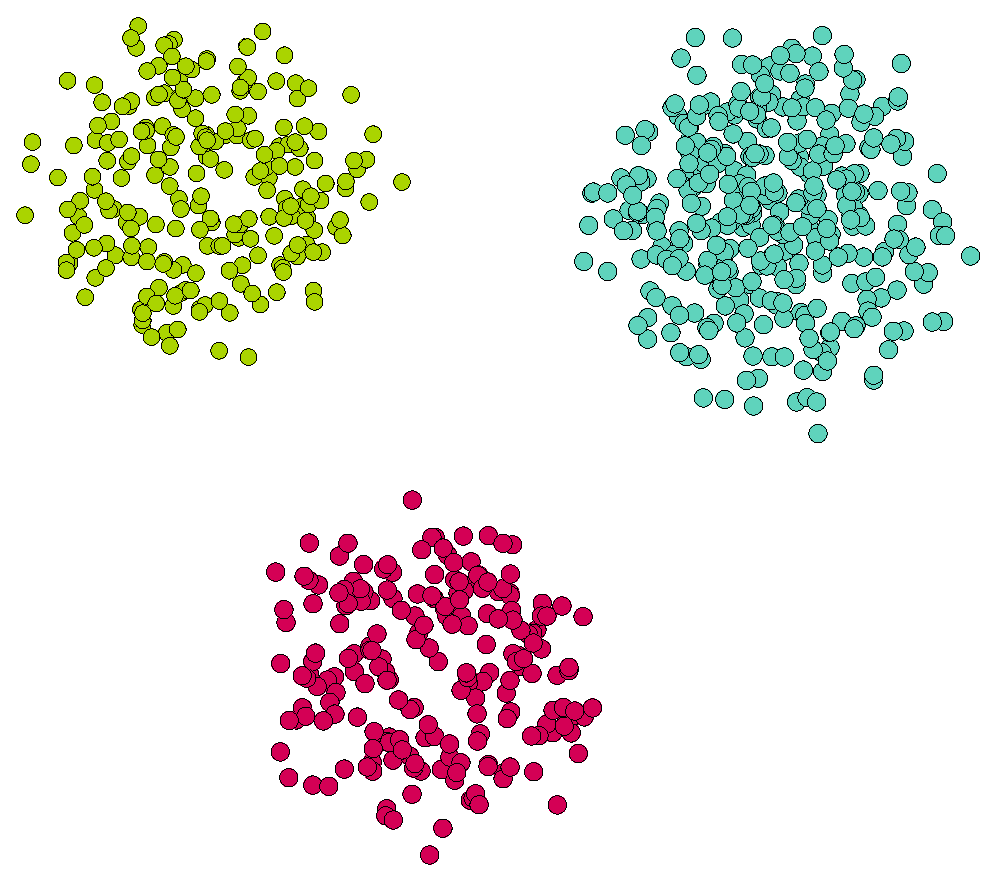
\includegraphics[width=.5\linewidth]{img/wellSeparatedObjects.eps}
  \caption{Dobře oddělené shluky}
  \label{fig:wellSeparatedObjects}
\end{subfigure}
\begin{subfigure}{.49\textwidth}
  \centering
  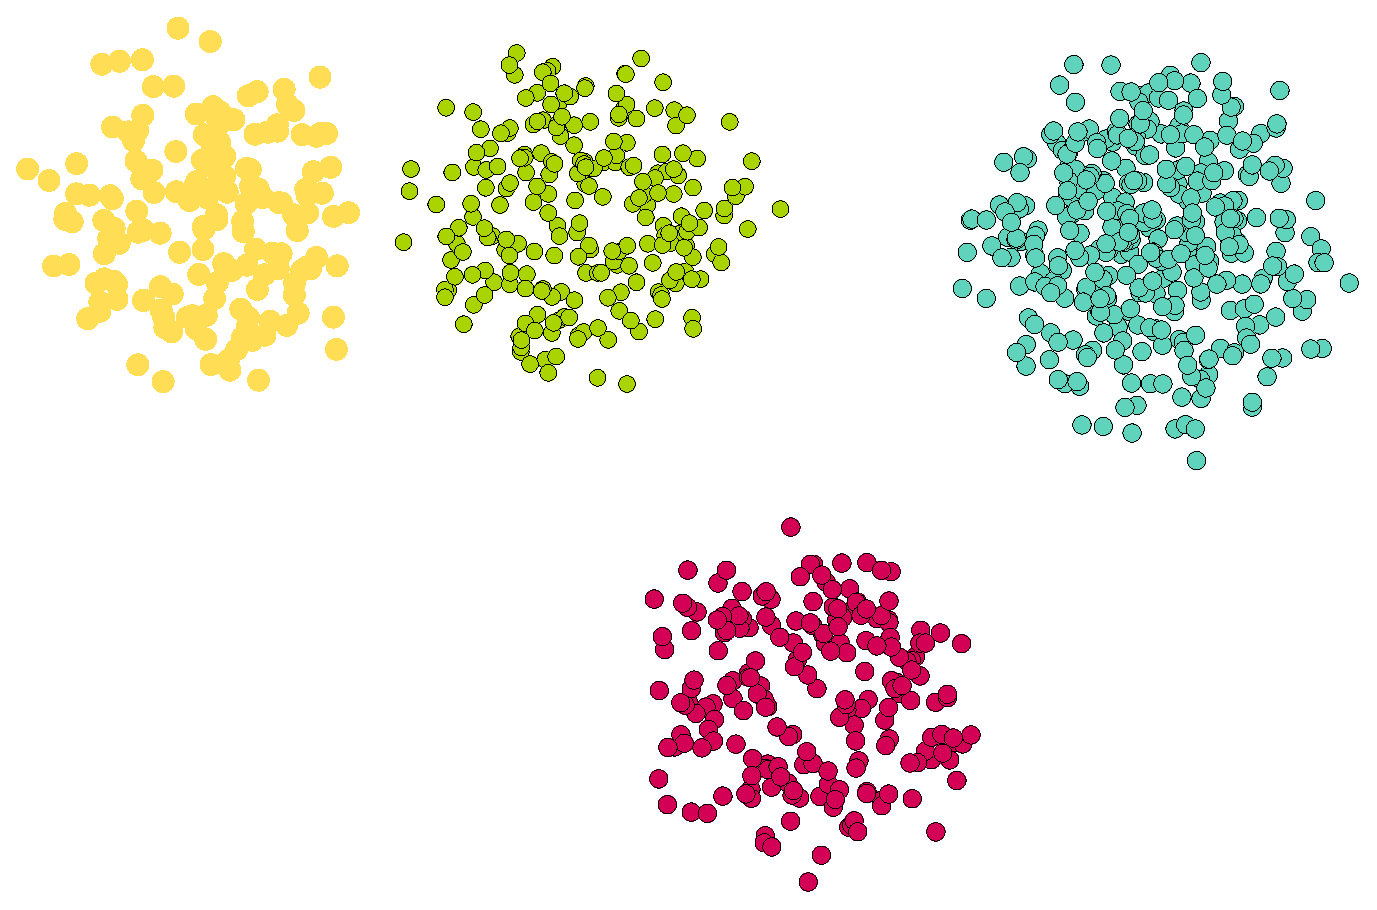
\includegraphics[width=.5\linewidth]{img/centerBasedClusters.eps}
  \caption{Shluky založené na centroidech}
  \label{fig:centerBasedClusters}
\end{subfigure}
\vspace*{0.5cm} 
\begin{subfigure}{.49\textwidth}
  \centering
  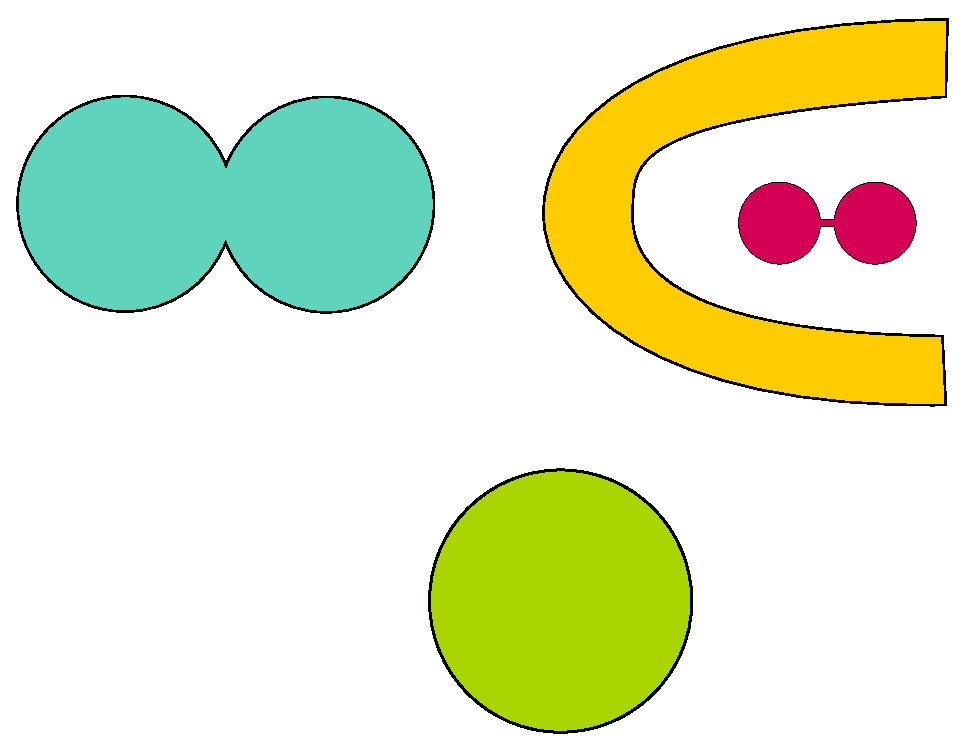
\includegraphics[width=.5\linewidth]{img/contiguousClusters.eps}
  \caption{Souvislé shluky}
  \label{fig:contiguousClusters}
\end{subfigure}
\begin{subfigure}{.49\textwidth}
  \centering
  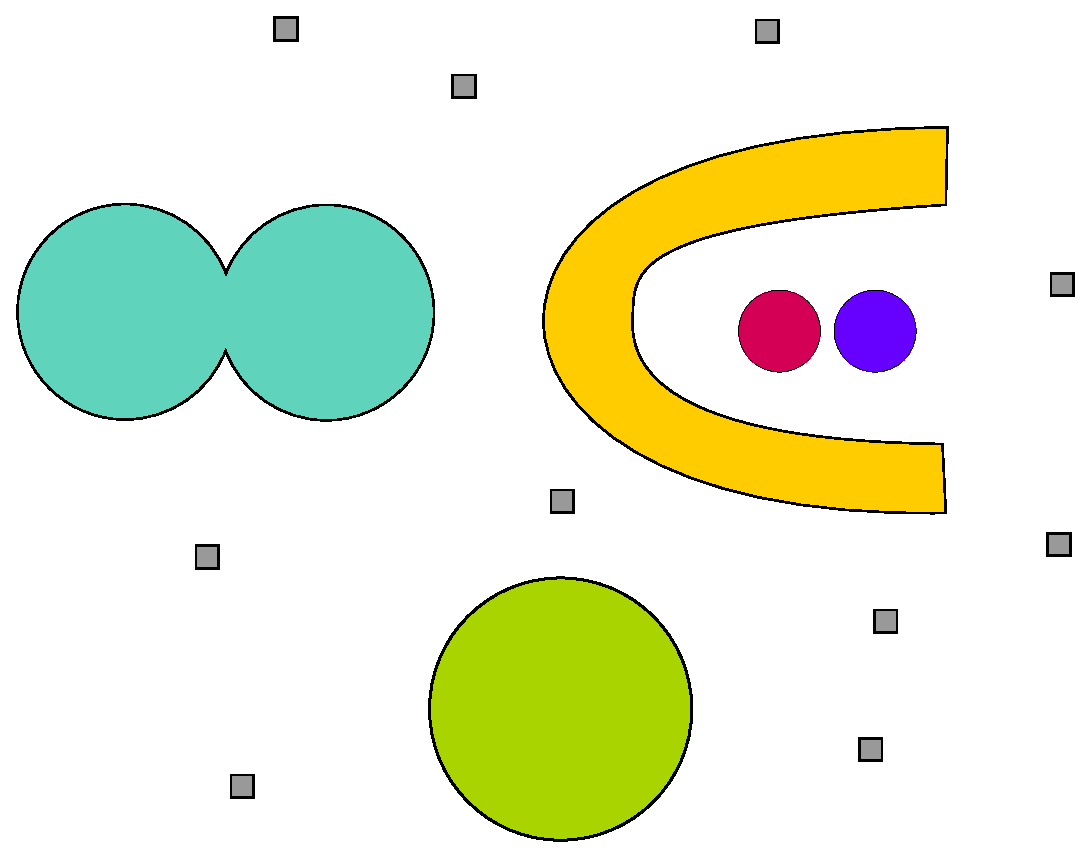
\includegraphics[width=.5\linewidth]{img/densityClusters.eps}
  \caption{Shluky založené na hustotě (šedé čtverečky představují šum)}
  \label{fig:densityClusters}
\end{subfigure}
\vspace*{0.5cm} 
\begin{subfigure}{.49\textwidth}
  \centering
  \includegraphics[width=.5\linewidth]{img/conceptualClusters.eps}
  \caption{Konceptuální shluky (Body ve shluku mají souřadnici y ze specifického rozsahu, ale souřadnice x se opomíjí)}
  \label{fig:conceptualClusters}
\end{subfigure}
\begin{subfigure}{.49\textwidth}
  \centering
  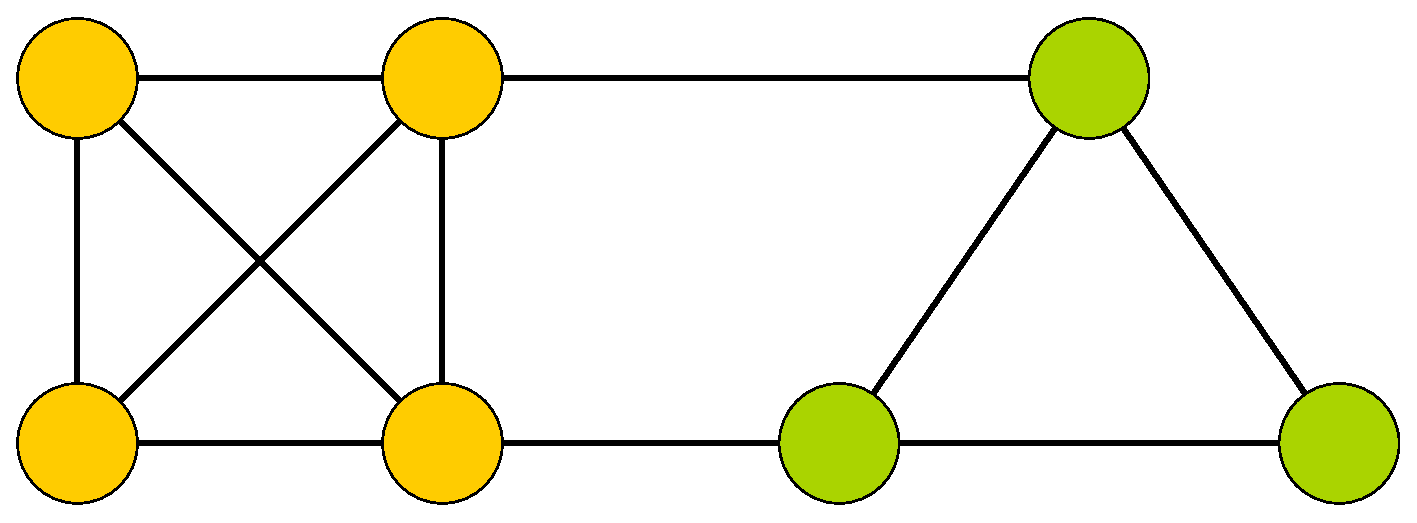
\includegraphics[width=.5\linewidth]{img/graphClusters.eps}
  \caption{Grafově orientované shluky}
  \label{fig:graphClusters}
\end{subfigure}
\caption{Typické modely shluků}
\end{figure}

\begin{description}
\item[Dobře oddělené shluky] Shluky jsou snadno oddělitelné - části shluků se ne\-pře\-krý\-va\-jí a~rozděluje je řídká nebo prázdná oblast. Shluk je množina objektů, kde je každý objekt uvnitř shluku bližší objektům z~jeho shluku než objektům z~jiných shluků~(\autoref{fig:wellSeparatedObjects}). Jedná se o~nejjednodušší vstup dat a~většina algoritmů v~tomto případě funguje dobře.

\item[Shluky založené na centroidech] Objekt patří do toho shluku, jehož centroidu (střed) je nejblíže~(\autoref{fig:centerBasedClusters}). Nevyžadujeme tedy oddělenost shluků jako u předchozího modelu. Centroid je speciální objekt vybraných nebo zkonstruovaný předtím, než se přiřazují objekty. Výsledek je podobný rozdělení prostoru do Voroného buněk, kde jsou shluky podobné právě Voroného buňkám z~Voroného diagramu. Centroidy jsou v tomto rozdělení nazývány generátory. Model založený na centroidech je vhodný pro algoritmy založené na vzdálenosti mezi objektem a~centroidem.\\

Jedním z~algoritmů pro řešení tohoto problému je \textbf{Centroidové shlukování}. Toto shlukování je optimalizačním problémem, kde hledáme centroidy tak, aby byla vzdálenost mezi body a~centroidy nejnižší. Problémem je, že samotná optimalizace je NP-těžký problém a~tak se často pro zjednodušení výpočtu optimální řešení pouze aproximuje. Aproximace se běžně provádí v~mnoha iteracích, které sestávají fáze přiřazení shluků k~objektům a~z fáze počítání nových centroidů.

\item[Souvislé shluky] Tento model je podobný modelu shluků založených na centroidech, ale rozdíl je v~tom, že pokud jsou dva shluky dostatečně blízko, mohou být spojeny do jednoho~(\autoref{fig:contiguousClusters}). Objekt tedy patří do shluku, pokud je podobný alespoň jednomu objektu z~daného shluku~\cite{Tan05}. \\

Hlavní myšlenka souvislých shluků je, že objekty, které jsou v~okolí, jsou více příbuzné než objekty, které jsou dále. Každý shluk tedy může být popsán například vzdáleností potřebnou pro připojení ke shluku. Mají-li shluky tuto vlastnost, můžeme je hierarchicky uspořádat tak, že nadřazené shluky jsou jen málo vzdálené od objektů v~nich obsažených. Tato hierarchie může být reprezentována jako dendrogram, což je stromový diagram zobrazující hierarchii shluků. Tato vlastnost může být použita jak pro hierarchické shlukování, tak pro pevné shlukování, pokud vynecháme hierarchické vlastnosti. \\

Propojování objektů do shluků může být problematické. Shluk totiž může obsahovat velké množství objektů a~je tedy mnoho možností, k~jakému objektu vzdálenost počítat. Mezi nejpoužívanější patří  vzdálenost mezi nejodlehlejšími nebo nejbližšími objekty dvou shluků, popřípadě vzdálenost průměrů nebo centroidů. %Existuje několik metod pro výběr kritérií propojení mezi dvěma množinami objektů $A$ a~$B$, $d$ je zvolená metrika:
%\begin{description}
%\item[Maximální nebo úplná vazba shluků] $$\max\{d(a,b) : a~\in A, b \in B\}$$
%\item[Minimální nebo jedinečná vazba shluků] $$\min\{d(a,b) : a~\in A, b \in B\}$$
%\item[Průměr, průměrná shluková vazba nebo UPGMA] (Unweighted Pair Group Method with Arithmetic Mean) $$\frac{1}{|A||B|}\sum_{a \in A} \sum_{b \in B} d(a,b)$$
%\item[Centroidová vazba shluků nebo UPGMC] (Unweighted Pair-Group Method using Centroids) $$\|c_a - c_b\| \mbox{ kde } c_a \mbox{ a } c_b \mbox{ jsou centroidy shluků } A \mbox{ a } B$$
%Toto může vypadat jako shlukování založené na centroidech, ale jde pouze o~kritérium vazby a~výsledkem jsou hierarchicky uspořádané shluky.
%\item[Minimální shluková energie] $$\frac{2}{|A||B|}\sum_{i,j=1}^{|A|,|B|}\|a_i-b_j\|_2-\frac{1}{n^2}\sum_{i,j=1}^{|A|}\|a_i-a_j\|_2-\frac{1}{|B|^2}\sum_{i,j=1}^{m}\|b_{i}-b_{j}\|_{2} : a \in A, b \in B$$
%\end{description}

%Tyto metody nejsou odolné proti extrémním objektům, které způsobují vytváření nových shluků nebo dokonce sloučení jiných. Metody mají obecně složitost $O(n^3) $, takže pro velké množství dat jsou pomalé. Pro speciální případy existují optimalizace, které mají jen složitost $O(n^2) $. Tyto metody jsou však považovány za zastaralé.

\item[Shluky založené na hustotě] Shluky jsou husté oblasti objektů oddělené oblastmi s~nízkou hustotou. Tato metoda je vhodná pro případy, kdy vstupní data obsahují šum, protože ten je pak odfiltrován oblastmi s~nízkou hustotou aniž by to změnilo rozdělení do shluků~(\autoref{fig:densityClusters}). Hustotu zde můžeme definovat jako počet objektů v jednotce prostoru.
Jedna z~nejpopulárnějších metod pro shlukování na základě hustoty je \textit{DBSCAN}. Jde o~podobnou metodu, jako je souvislé shlukování, protože spojuje body na základě vzdálenosti. Liší se ale v~tom, že spojuje pouze body splňující kritérium hustoty. To znamená, že v~okolí určeném vzdáleností musí být alespoň minimální počet objektů. Tyto objekty se pak nazývají jádro a~vytváří základ shluku. Objekty, které nesplňují kritérium hustoty, ale jsou dostatečně blízko k~alespoň jednomu bodu ze shluku, se přidávají do shluku.
Výhodou této metody je její výpočetní nenáročnost, protože vyžaduje pouze lineární počet dotazů na rozsah. Tato metoda je navíc deterministická, takže ji není potřeba spouštět v~iteracích.
Nevýhodou této metody je parametr hustoty $\epsilon$, protože při špatném nastavení mohou být hranice shluků s~menší hustotou interpretovány jako šum. Problémy způsobují také shluky, které leží blízko sebe, protože mohou být chápány jako jeden.

\item[Distribuční modely shluků] Shluky v~distribučních modelech jsou objekty, kte\-ré patří ke stejné distribuci pravděpodobnosti. Model umožňuje, aby jeden objekt patřil do více shluků a tedy i do více distribucí.
Tento přístup v~podstatě napodobuje proces generování vstupních dat a~sna\-ží se rekonstruovat ztracené statistické parametry. %Hlavní problém tohoto modelu shluků je problém známý jako \textit{overfitting}, což znamená, že komplexnější model je popsán méně složitým a~rozdíl mezi nimi je označen jako odchylka nebo šum. Například 3 body z~okolí vrcholu paraboly budou popsány lineární funkcí.
Jednou z~metod používaných v~distribučním shlukování je \textit {Gaussian mixture models}, kde algoritmus iterativně optimalizuje parametry pevného počtu Gaussových distribucí.
Tato metoda předpokládá vstupní množinu s~daty odpovídajícími Gaussově distribuci, ale problémem je, že data nemusí od\-po\-ví\-dat vůbec žádné distribuci a~tedy nemusí mít ani žádný model.

\item[Konceptuální shluky] Objekty uvnitř shluku mají některé vlastnosti stejné nebo podobné, ale jiné vlastnosti se mohou významně lišit~(\autoref{fig:conceptualClusters}). Je to dáno tím, že při konceptuálním shlukování známe význam a jednotlivých vlastností. Tím pádem můžeme důležité vlastnosti upřednostnit a jiné naopak upozadit.
Jako algoritmus pro konceptuální shluky můžeme použít algoritmus, který závisí na jen na podstatných vlastnostech modelu a~méně významné vlastnosti objektů jednoduše ignoruje.

\item[Grafově orientované shluky] Shluky mohou být definovány například jako kli\-ky v~grafech. Klika je podmnožina uzlů, kde je každý uzel spojen hranou s~ostatními vrcholy v~klice~(\autoref{fig:graphClusters}).
Kvůli speciálním požadavkům tohoto modelu jsou zapotřebí speciální algoritmy, jako je například algoritmus Bron-Kerbosch ~\cite{Sun15} pro nalezení klik.
\end{description}

\section{Další využití shlukové analýzy} \label{sec:otherdata}
Pro zajímavost uvádíme příklady využití shlukové analýzy nad nevektorovými prostory.

\subsection{Statistická data}
Pokud cheme shlukovat data nad množinami dat na základě jejich statistických vlastností, můžeme využít funkcí jako je \textbf{Mahalanobisova vzdálenost} a~\textbf{Wassersteinova metrika}

\subsubsection{Mahalanobisova vzdálenost}
Je užitečná, pokud potřebujeme zjistit pravděpodobnostní vzdálenost skupin objektů nebo vzdálenost objektu od skupiny. Při počítání vzdálenosti bere v úvahu korelaci mezi statistickými parametry a navíc je nezávislá na rozsahu hodnot. Hlavní myšlenkou této vzdálenosti je měření odlišnosti objektu $P$ od průměru skupiny $D$.
Pokud máme pozorování $p = (p_1,..., p_n)^T$ a~střední hodnotu pozorování $\mu=(\mu_1,...,\mu_n)^T $ a~matici kovariance $S$, Mahalanobisova vzdálenost je definována jako:
$$D_M(x) = \sqrt{(x - \mu)^T S^{-1} (x-\mu)}$$

\subsubsection{Wassersteinova metrika}
Další vzdálenost použitá ve statistice je Wassersteinova metrika (nazývaná též Earth mover's distance (EMD))~\cite{Vallender73}. Tato metrika se používá pro výpočet vzdá\-le\-nos\-ti mezi dvěma pravděpodobnostními distribucemi na daném metrickém prostoru $M$. Jak název napovídá, název vznikl díky analogii s~posouváním "zeminy" nahromaděné stejným způsobem, jako je tvar distribuce pravděpodobnosti. Vzdálenost je množství zeminy, které musí být přemístěno tak, aby se změnil tvar hromady na jiný tvar určený rozložením druhé pravděpodobnosti. Množství je pak ještě potřeba vynásobit vzdáleností, o~kterou je třeba zeminu přesunout.%Tato vzdálenost je definována takto: \\
%Nechť $X$ je metrický prostor s~metrikou $\rho$ a~$\mathfrak {B}$ je $\sigma$-algebra Borelovských podmnožin $X$. Wassersteinova vzdálenost $R(P, Q)$ mezi rozdělení pravděpodobnosti $P$ a~$Q$ na $(X, \mathfrak{B}) $ je definována jako:
%$$R(P,Q)=\inf\mathbf{E}\rho(\xi, \sigma)$$
%kde $\inf$ se bere  ze všech možných dvojic náhodných proměnných $\xi$ a~$\sigma$ s~distribucí $P$ a~$Q$.\\

\subsection{Nečíselná data}
Existují také prostory, které nemají s~matematikou mnoho společného, ale obsahují objekty, které jsou porovnatelné.

\subsubsection{Levenshteinova vzdálenost} Levenshteinova vzdálenost se používá k~výpočtu editační vzdálenosti mezi dvěma řetězci $ a, b $ a~je rekurzivně definována takto:
\begin{equation*}
lev_{a,b}(i,j)=
\begin{cases}
max(i,j) & $pokud $ min(i,j)=0, \cr
min \begin{cases}
lev_{a,b}(i-1,j) + 1 \cr
lev_{a,b}(i,j-1) + 1 \cr
lev_{a,b}(i-1,j-1) + dif(a_i,b_j)
\end{cases} & $jinak$
\end{cases}
\end{equation*}
kde \begin{equation*}
dif(a_i,b_j)=
\begin{cases}
0 & $pokud $ a_i = b_j, \cr
1 & $jinak$
\end{cases}
\end{equation*}

$a_i, b_j$ značí i-tý znak řetězce $a$ respektive j-tý znak řetězce $b$.

\subsubsection{Signature Quadratic Form Distance}
Tato metrika se používá pro porovnávání multimediálních objektů, které mohou být popsány různými charakteristikami. Problém je v~tom, že se tyto charakteristiky mohou lišit ve struktuře a~velikosti, takže nemůžeme použít běžné vzdálenosti. Vlastnost každého objektu je popsána vektorem dvojic centroidů z~prostoru vlastností $\mathbb{FS}$ a~jeho váhy z~$\mathbb{R^{+}}$.
Nepočítáme tedy vzdálenosti mezi vlastnostmi, ale právě pomocí Signature Quadratic Form Distance~\cite{Beecks10}, kde používáme funkce podobnosti.
Matematicky je Signature Quadratic Form Distance (SQFD) definovaná pro dvě množiny vlastností $S^{q} = \{\{c_i^q, w_i^q\}|i=1,...,n\}$ and $S^{o} = \{\{c_i^o, w_i^o\}|i=1,...,m\}$ a~funkce podobnosti $f_s(c_i, c_j)\to \mathbb{R}$ takto:
$$SQFD_{f_s}(S^q,S^o)=\sqrt{(w_q|-w_o)A_{f_n}(w_q|-w_o)^T}$$
Kde $A_{f_n} \in \mathbb{R}^{(n+m)\times(n+m)}$ je matice podobnosti vygenerovaná aplikací funkce podobnosti $f_s$ na odpovídající centroidy  ($a_{ij}=f_s(c_i,c_j)$) a~operátor $|$ znamená zřetězení dvou vektorů, takže $w_q|-w_o = (w_1^q,...,w_n^q,-w_1^o,...,-w_m^o)$\\

\section{K-Means}
Pokud chceme urychlit jakýkoliv algoritmus co nejefektivněji, musíme využít každý jeho detail. To ovšem není možné udělat obecně pro všechny algoritmy shlukové analýzy a je tedy potřeba zaměřit se na konkrétní algoritmus. Na druhou stranu je také potřeba zvolit dostatečně obecný algoritmus, aby byl výsledek co nejpoužitelnější. Jako vhodného reprezentanta jsme se rozhodli zvolit algoritmus k-means kvůli jeho široké škále využití a~nezávislosti na vlastnostech vstupních dat. \\

\subsection{Definice}
K-means algoritmus~\cite{Aggarwal13, Tan05} je algoritmus využívající shlukový model založený na centroidech. Vstupem je množina $n$ bodů v~$d$-dimenzionálním prostoru $R^d$, počet výstupních shluků $k$ a~počtu iterací $i$.
Úkolem je jednotlivé body přiřadit k centroidům (středům shluků) a vytvořit tak shluky. Toto rozdělení se navíc snažíme optimalizovat tak, aby byla suma vzdáleností mezi jednotlivými body a přiřazenými centroidy co nejmenší. Algoritmus funguje iterativně a~každá i\-te\-ra\-ce se skládá ze dvou kroků. V~prvním kroku je pro každý bod nalezen nejbližší centroid. Tento bod je přidělen do shluku, který k~centroidu náleží. Ve druhém kroku jsou nové centroidy vypočítány jako průměr (mean) všech bodů přidělených stej\-né\-mu shluku. Algoritmus končí po předem daném počtu kroků nebo pokud se mezi dvěma iteracemi nezmění rozdělení bodů do shluků.
Výstupem tohoto algoritmu jsou souřadnice centroidů a~případně i~body rozdělené do shluků.

\algdef{SE}[REPEAT]{Repat}{Until}{\algorithmicrepeat}[1]{\algorithmicuntil\ #1}

\begin{algorithm}
\caption{K-means}\label{alg:kmeans}
\begin{algorithmic}[1]
\State Vyber K~bodů jako iniciální centroidy
\Repeat
\State Vytvoř K~shluků přiřazením bodů k~nejbližším centroidům
\State Aktualizuj centroidy
\Until{centroidy se nezměnily nebo bylo dosaženo maximálního počtu iterací}
\end{algorithmic}
\end{algorithm}

Protože v~prvním kroku neznáme centroidy, často se jako počáteční hodnoty používá prvních $k$ bodů vstupní množiny. Algoritmus K-means konverguje rychle během několika prvních iterací, takže můžeme definici pozměnit tak, že se algoritmus zastaví, pokud mezi dvěma iteracemi dojde ke změně pouze $\epsilon$ centroidů. kde $\epsilon$ je předem dané. \cite{Tan05}.
Složitost výpočtu je $O(n\times k\times i\times d)$, kde $n$ je počet vstupních bodů, $k$ je počet clusterů, $i$ je počet iterací a~$d$ je dimenze vstupních dat. \\

\subsection{Měření kvality}
Abychom mohli vyhodnotit výstup k-means, musíme umět měřit kvalitu přiřazení do shluků. Pro tento účel se nejčastěji používá funkce \textbf{Sum of Squared Error (SSE)}. Chyba jednoho bodu je reprezentována vzdáleností od centroidu daného shluku a~funkce SSE pak sčítá čtverce chyb jednotlivých bodů.
$$SSE = \sum^k_{i=1}\sum_{o \in O_i}|o,c_i|^2, \textrm{ $c_i$ \textit{je středem shluku} $O_i$ }$$
Pokud dostáváme výsledky s vysokým $SSE$, můžeme jej snížit například zvýšením počtu shluků $k$. Pokud jsou ale počáteční shluky vybrány špatně, nemusí ani zvýšení počtu shluků pomoci a je potřeba vybrat jiné počáteční centroidy (změnit algoritmus výběru).\\

\subsection{Omezení k-means} \label{ssec:kmeansrestrictions}
Pevný počet počátečních centroidů je jednou z~nevýhod k-means algoritmu, protože jej potřebujeme znát již na začátku a~v~základní variantě k-means už toto číslo nelze změnit během výpočtu. Tuto možnost mohou ale některé typy problémů vyžadovat a~tak jsou pro ně k-means nepoužitelné.  I~když zvolíme ideální $k$ pro vstupní data, dostaneme se k dalšímu problému, kterým je výběr počátečních centroidů. V ideálním případě jsou totiž počáteční centroidy každý z~jiného shluku, ale pravděpodobnost, že jsme objekty zvolili právě takto, je opravdu malá~\cite{Tan05}: $$P = \frac{\mbox{počet možností výběru jednoho bodu z~každého shluku}}{\mbox{počet možností volby K~centroidů}}=\frac{k!{n \choose k}}{k^k {n \choose k} }=\frac{k!}{k^k}$$ Tato pravděpodobnost se blíží nule i~pro relativně malé $k$. Například pro $k=10$, je pravděpodobnost $0.00036$. \\

Existují ale způsoby, jak tento problém vyřešit a~vybrat lepší počáteční body~\cite{Tan05}:
\begin{description}
\item[více běhů] k-means je spuštěn několikrát s~různými počátečními body a~jako výstup je vybrán nejlepší výsledek. To nemusí vést k ideálnímu výběru iniciálních centroidů, protože pokud bychom chtěli mít alespoň 50\% šanci, že je vybereme, museli bychom pro hodnoty z příkladu udělat skoro 2000 běhů ($1 - (1 - 0.00036)^2000 \doteq 0.51$). Pokud ale spustíme algoritmus vícekrát s různými počátečními centroidy, můžeme vybrat lepší řešení.
\item[vzorkování] Počáteční centroidy jsou vybrány na základě vzorkování vstupních dat hierarchickým shlukování.
\item[více centroidů] Je vybráno více centroidů než je vstupní $k$ a~z nich se vyberou ty nejlépe rozmístěné.
\item[následné zpracování] Výsledek algoritmu je následné zpracován - Shluky s~nej\-vyš\-ším $SSE$ jsou rozděleny a~na druhou stranu shluky s~nejnižším $SSE$ mohou být spojeny.
\end{description} 

Dalším problémem k-means je, že základní verze může produkovat i~prázdné shluky~(\autoref{fig:kmeansemptycluster}). To lze vyřešit úpravou algoritmu: pokud najdeme prázdný shluk, můžeme ho nahradit bodem, který nejvíce přispívá k~$SSE$. Další možností je vybrat bod z~clusteru s~největším $SSE$ ~\cite{Tan05}.\\

\begin{figure}[h]
\centering
\begin{subfigure}{.49\textwidth}
  \centering
  \includegraphics[width=.9\linewidth]{img/kmeans_emptyCluster1.eps}
  \caption{Vstupní data}
  \label{fig:kmeansemptycluster1}
\end{subfigure}
\begin{subfigure}{.49\textwidth}
  \centering
  \includegraphics[width=.9\linewidth]{img/kmeans_emptyCluster2.eps}
  \caption{Jako iniciální centroidy zvolíme body 1,2,3}
  \label{fig:kmeansemptycluster2}
\end{subfigure}
\vspace*{0.5cm} 
\begin{subfigure}{.49\textwidth}
  \centering
  \includegraphics[width=.9\linewidth]{img/kmeans_emptyCluster3.eps}
  \caption{Přiřazení ke clusterům a výpočet nových (vzdálenost mezi 1 a 7 je větší než mezi 2 a 7)}
  \label{fig:kmeansemptycluster3}
\end{subfigure}
\begin{subfigure}{.49\textwidth}
  \centering
  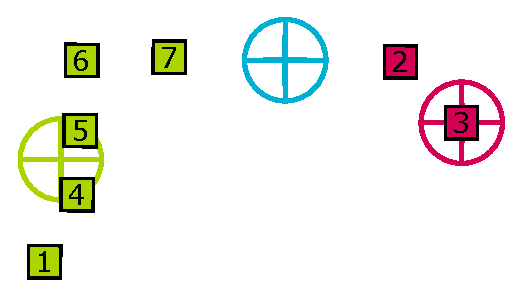
\includegraphics[width=.9\linewidth]{img/kmeans_emptyCluster4.eps}
  \caption{Vznik prázdného clusteru (7 je blíže k zelenému centroidu, 2 blíže k růžovému)}
  \label{fig:kmeansemptycluster4}
\end{subfigure}
\caption{Prázdný shluk}
\label{fig:kmeansemptycluster}
\end{figure}

\subsection{Nevhodná data}
Problematická mohou být také vstupní data. Pokud se shluky výrazně liší v~rozměrech/hustotě nebo jde-li o~nekulovité útvary, má pak shluková analýza problém s~nalezením centroidů~\cite{Tan05}. \\

Jelikož hlavním cílem k-means je nalézt shluky s~podobnou velikostí, budeme mít problém se vstupními daty, které obsahují jeden velký shluk s~mnoha objekty a~jeden menší shluk s~několika málo objekty~(\autoref{fig:kmeansbadinputsize}). K-means potom rozdělí větší shluk~(\autoref{fig:kmeansbadoutputsize}), takže objekty, které náleží logicky do většího shluku, ale zároveň jsou blíže centroidu z~menšímu shluku, jsou přiřazeny k~menšímu shluku, což může být nežádoucí. Je to dáno tím, že k-means ignorují distribuci vstupních dat.

\begin{figure}[h]
\centering
\begin{subfigure}{.49\textwidth}
  \centering
  \includegraphics[width=.5\linewidth]{img/kmeans_badInputSampleSize.eps}
  \caption{Vstupní data (rozřazené do shluků jen pro ilustraci)}
  \label{fig:kmeansbadinputsize}
\end{subfigure}
\begin{subfigure}{.49\textwidth}
  \centering
  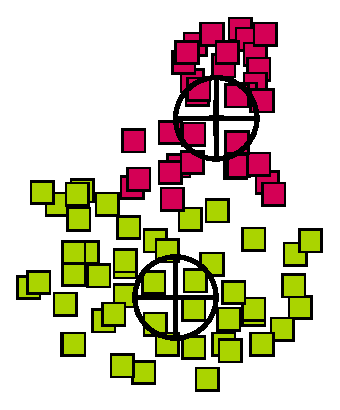
\includegraphics[width=.5\linewidth]{img/kmeans_badOutputSampleSize.eps}
  \caption{výstup k-means}
  \label{fig:kmeansbadoutputsize}
\end{subfigure}
\caption{K-means nad shluky různých velikostí}
\end{figure}

Také hustota shluků může způsobovat k-means problémy. Když máme dva husté shluky blízko sebe a~jeden vzdálenější shluk s~nízkou hustotou~(\autoref{fig:kmeansbadinputdensity}), k-means obvykle označují husté shluky jako jeden a~rozdělí řídký shluk do více shluků~(\autoref{fig:kmeansbadoutputdensity}).
\begin{figure}[h]
\begin{subfigure}{.49\textwidth}
  \centering
  \includegraphics[width=.5\linewidth]{img/kmeans_badInputSampleDensity.eps}
  \caption{Vstupní data (rozřazené do shluků jen pro ilustraci)}
  \label{fig:kmeansbadinputdensity}
\end{subfigure}
\begin{subfigure}{.49\textwidth}
  \centering
  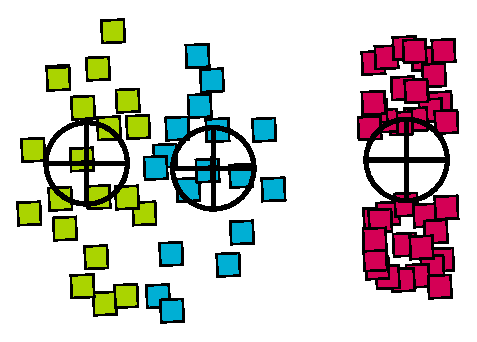
\includegraphics[width=.5\linewidth]{img/kmeans_badOutputSampleDensity.eps}
  \caption{výstup k-means}
  \label{fig:kmeansbadoutputdensity}
\end{subfigure}
\caption{K-means nad shluky různé hustoty}
\end{figure}

Další nevýhodou k-means je, že algoritmus nerozpozná tvar shluku a~produkuje pouze kulové shluky. To je problém, pokud dva obvykle nekonvexní shluky~(\autoref{fig:kmeansbadinputshape}) jsou dostatečně blízko a~jeden zasahuje do konvexního obalu toho druhého. K-means pak obvykle přidělují body z~jednoho shluku do druhého a~naopak~(\autoref{fig:kmeansbadoutputshape}).\\
\begin{figure}[h]
\begin{subfigure}{.49\textwidth}
  \centering
  \includegraphics[width=.5\linewidth]{img/kmeans_badInputSampleShape.eps}
  \caption{Vstupní data (rozřazené do shluků jen pro ilustraci)}
  \label{fig:kmeansbadinputshape}
\end{subfigure}
\begin{subfigure}{.49\textwidth}
  \centering
  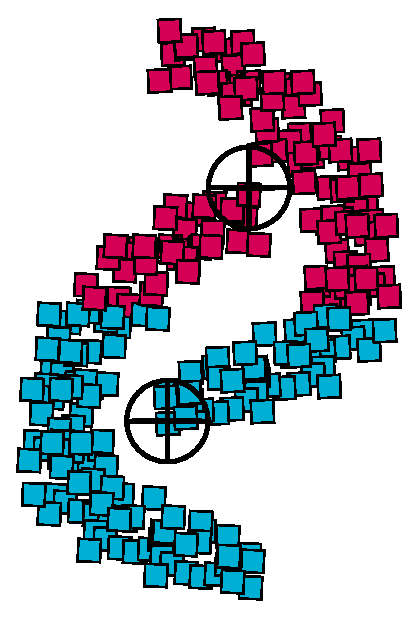
\includegraphics[width=.5\linewidth]{img/kmeans_badOutputSampleShape.eps}
  \caption{výstup k-means}
  \label{fig:kmeansbadoutputshape}
\end{subfigure}
\caption{K-means nad nekulovitými shluky}
\end{figure}

Tyto problémy mohou být vyřešeny použitím více shluků, než přirozeně vyžadují vstupní data. Například vstupní data~(\autoref{fig:kmeansbadinputshape}) obsahují dva přirozené shluky, ale když se pokusíme rozdělit data na více shluků, výsledek bude obsahovat malé shluky, které obsahují body z~jednoho přirozeného shluku a~neobsahují shluky z~druhého~(\autoref{fig:kmeansbadoutputsolution}). Pokud tyto informace následně zpracujeme, můžeme získat očekávaný výsledek a~napravit tak tento nedostatek k-means.
\begin{figure}[h]
  \centering
  \includegraphics[width=.3\textwidth]{img/kmeans_badOutputSampleShapeSolution.eps}
  \caption{řešení k-means pro shluky špatných tvarů}
  \label{fig:kmeansbadoutputsolution}
\end{figure}


\subsection{Varianty k-means}
Protože k-means jsou univerzálním algoritmem, existují různé varianty pro případy, kdy je klasický algoritmus k-means nevhodný nebo nepoužitelný. Tyto varianty mohou vyřešit některé problémy a~omezení klasického algoritmu k-means.
\begin{description}
\item[k-medoids] - centroidy nejsou uměle vytvořené objekty v~prostoru vstupních dat, ale reálné objekty ze vstupu (medoidy nebo exepláře). Na rozdíl od k-means se zde nesnažíme minimalizovat celkovou vzdálenost, ale součet odchylek mezi objekty shluku a objektu vybraného jako střed shluku.
\item[k-medians] - stejný algoritmus jako k-means, ale pro výpočet nového centroidu se pro každou dimenzi využívá medián místo výpočtu průměrné hodnoty. Hodnoty v jednotlivých dimenzích jsou tedy reálné hodnoty ze vstupních dat, ale celý objekt ve vstupních datech nemusí být vůbec obsažen.
\item[k-means++] - Počáteční centroidy jsou vybrány náhodně. Tím lze zabránit potenciálním špatným vstupům.
\item[Fuzzy K-means] - jsou povoleny neostré shluky~(\autoref{sec:clusterorganization}). Objekty nepatří striktně jednomu shluku, ale využíváme stupeň náležení k~jednotlivým shlukům. Pro výpočet nových centroidů se využívá vážený průměr (kde je jako váha brán stupeň náležení).
\item[Rozdělující (Bisecting) k-means]~\cite{Tan05} je varianta k-means, která produkuje hierarchické uspořádání shluků. Pracuje, stejně jako k-means, iterativně, ale v~každém kroku je shluk s~nejvyšším $SSE$ rozdělen na 2 pomocí klasického k-means algoritmu s~parametrem $k=2$. \autoref{alg:bisectingkmeans} iteruje, dokud nedosáhne daného počtu shluků.
\begin{algorithm}
\caption{Rozdělující k-means}\label{alg:bisectingkmeans}
\begin{algorithmic}[1]
\State Vlož všechny body do seznamu shluků jako jeden shluk
\Repeat
\State Vyber první shluk ze seznamu shluků
\For{i=1 do daného počtu iterací}
\State Rozděl vybraný shluk pomocí základního k-means algoritmu
\EndFor
\State Přidej dva shluky vzniklé rozdělením s~nejnižším SSE do seznamu shluků
\State Aktualizuj centroidy pro každý shluk
\Until{seznam shluků obsahuje k~shluků}
\end{algorithmic}
\end{algorithm}

\end{description}

\subsection{Optimalizace a heuristiky implementace K-means} \label{ssec:optimization}
Stejně jako většina jiných algoritmů, i u k-means při bližším zkoumání nalezneme při implementování místa, kde lze algoritmus optimalizovat nebo zrychlit pomocí heuristik.
Zaměříme se tedy na jednotlivé kroky algoritmu k-means~\ref{alg:kmeans}

\subsubsection{Inicializace}
Hned první možností pro vylepšení je inicializace algoritmu, konkrétně výběr počátečních centroidů. Pokud se nám totiž podaří program dobře inicializovat, vyhneme se velkému množství iterací. Středy shluků jsou v základní verzi vybrány tak, že se vezme prvních $n$ bodů ze vstupu a prohlásíme je za středy budoucích clusterů. Může se tak stát, že pro nevhodná data zvolíme všechny body z jednoho shluku a tím pádem budeme muset provést více iterací, než dojdeme k výsledku. Ideální případ, jak již bylo napsáno výše v sekci~\ref{ssec:kmeansrestrictions}, je vybrat body z různých shluků, ale pravděpodobnost takového výběru je velice malá. Je tedy potřeba zvolit vhodnou heuristiku pro výběr počátečních clusterů.\\% K tomu se často využívají k-dimenzionální stromy.

Jednu z prvních metod, jak počáteční body vybrat, navrhl Forgy v roce 1965~\cite{Anderberg73}. Jeho myšlenka spočívá jednoduše v tom, že jsou body vybrány náhodně ze vstupních dat. Pokud centroidy zvolíme takto, je větší šance, že to budou v blízkosti středů reálných shluků, protože jde o místa s největší hustotou bodů. Není zde ale žádná záruka, že nezvolíme 2 body ze stejného shluku a nebo že nezvolíme odlehlý bod. I přes své nevýhody se ale Forgyho metoda standardně používá ve spojení s vícenásobným spuštěním.\\

S další metodou přišel v roce 1967 J. B. MacQueen~\cite{MacQueen67}. Jeho metoda je podobná Forgyho přístupu. Na začátku se také vyberou náhodné body ze vstupních dat jako počáteční centroidy, ale pak se místo rozřazení všech bodů do shluků a iterování k výsledku postupuje jinak. V každém kroku vezmeme následující bod ze vstupu a přiřadíme ho k nejbližšímu centroidu. Poté spustíme k-means, čímž se nám centroidy změní, a teprve pak začneme zpracovávat další bod. Problém tohoto přístupu je samozřejmě ve výpočetní složitosti, protože se k-means spouští pro každý bod, což je pro velká vstupní data velice náročné.\\

\subsubsection{k-dimenzinální stromy}
k-dimenzinální stromy (nebo kd-stromy) jsou strukturou určenou pro ukládání vícerozměrných dat. Jde o binární strom, kde každý uzel reprezentuje podmnožinu bodů a jeho potomci pak tuto podmnožinu rozdělují na disjunktní podmnožiny. Dělení probíhá tak, že spočítáme medián dimenze $d$ ze všech bodů v intervalu reprezentovaném uzlem. V levém potomkovi jsou pak body s menší hodnotou v dimenzi $d$, v pravém pak s větší hodnotou. Na každé hladině se střídá dimenze, podle které body dělíme až nakonec v listech jsou pouze množiny obsahující jednotlivé body. V každém volání funkce kdTree v~algoritmu~\ref{alg:kdtreeconstruction} se body rozdělí na polovinu. Počet volání funkce je tedy $\log_2(n)$. Výběr mediánu lze zvládnout v čase $\mathcal{O}(n)$ díky podobném triku jako například v algoritmu Quicksort~\cite{Cormen07}. Roztřízení bodů je pak také v čase $\mathcal{O}(n)$. Celková složitost konstrukce kd-stromu je tedy $\mathcal{O}(n \log(n))$.

\begin{algorithm}
\caption{Konstrukce kd-stromu}\label{alg:kdtreeconstruction}
\begin{algorithmic}[1]
\Function{kdTree}{bodyKRozdělení, hloubka}
\State Pokud velikost(bodyKRozdělení) = 1, vrať list
\State Vyber rozdělující dimenzi d podle hloubky
\State Vyber medián m z d-té dimenze v bodyKRozdělení
\State levý syn = kdtree(body b z bodyKrozdělení kde b[d] < m, hloubka++)
\State pravý syn = kdtree(body b z bodyKrozdělení kde n[d] > m, hloubka++)
\State vrať zkonstruovaný bod
\EndFunction
\end{algorithmic}
\end{algorithm}

Pro využití kd-stromu v algoritmu k-means nemusíme stavět celý strom, což by bylo velice náročné, ale stačí nám rozdělit body do tolika podmnožin, abychom z každé z nich mohli vybrat jeden počáteční centroid. Pokusy ukazují, že výběr iniciálních bodů pomocí kd-stromů je efektivnější, než náhodný výběr~\cite{Pahala10}.
